\chapter{Appendix: HpCom Code Examples}

% \section{Architecture}

% Some

\section{Defining the Parameters}
\label{sec:hpcom_param}

The following list details the elements of the WDM parameters dictionary created by the \texttt{create\_wdm\_parameters} function:

\begin{description}[style=multiline, leftmargin=4cm, font=\normalfont]
    \item[\texttt{n\_channels}] Number of Wavelength Division Multiplexing channels.
    \item[\texttt{channel\_spacing}] Channel spacing in Hz.
    \item[\texttt{n\_polarisations}] Number of polarizations.
    \item[\texttt{p\_ave\_dbm}] Average power in dBm.
    \item[\texttt{n\_symbols}] Number of symbols.
    \item[\texttt{m\_order}] Modulation order.
    \item[\texttt{modulation\_type}] Type of modulation, derived from modulation order.
    \item[\texttt{n\_bits\_symbol}] Number of bits per symbol, derived from modulation type.
    \item[\texttt{roll\_off}] Roll-off factor for Root Raised Cosine filter.
    \item[\texttt{upsampling}] Upsampling factor.
    \item[\texttt{downsampling\_rate}] Downsampling rate.
    \item[\texttt{symb\_freq}] Symbol frequency in Hz.
    \item[\texttt{sample\_freq}] Sampling frequency in Hz, calculated as the product of symbol frequency and upsampling factor.
    \item[\texttt{np\_filter}] Nyquist pulse filtering.
    \item[\texttt{p\_ave}] Average power in Watts, calculated from \texttt{p\_ave\_dbm}.
    \item[\texttt{seed}] Seed for random number generator.
    \item[\texttt{scale\_coef}] Scale coefficient for constellation, derived based on modulation type, average power, and number of polarizations.
\end{description}

Below is an example of how the \texttt{create\_wdm\_parameters} function can be used with some specific parameters:

\begin{lstlisting}[language=Python, caption=Usage of create\_wdm\_parameters function, label=lst:create_wdm_param]
# Import the function
from hpcom.signal import create_wdm_parameters

# Define the parameters
n_channels = 4
p_ave_dbm = -3
n_symbols = 2**15
m_order = 16
roll_off = 0.2
upsampling = 4
downsampling_rate = 2
symb_freq = 32e9
channel_spacing = 50e9

# Call the function
wdm_params = create_wdm_parameters(
    n_channels, p_ave_dbm, n_symbols, m_order, 
    roll_off, upsampling, downsampling_rate, 
    symb_freq, channel_spacing
)

# Now wdm_params contains the WDM parameters dictionary
\end{lstlisting}

In example~\ref{lst:create_wdm_param}, the \texttt{create\_wdm\_parameters} function is called with specific values for the parameters, and the resulting dictionary is stored in the \texttt{wdm\_params} variable.

The functions \texttt{get\_default\_wdm\_parameters} and \texttt{get\_default\_channel\_parameters} furnish the capability to generate default parameters for \Gls{wdm} signal creation and \gls{ssmf} channel with \gls{edfa} amplification, respectively.

\begin{lstlisting}[language=Python, caption=Default WDM parameters, label=lst:default_wdm_param]
def get_default_wdm_parameters():

 wdm = {}
 wdm['n_channels'] = 1  # Single WDM channel
 wdm['channel_spacing'] = 75e9  # 75 GHz
 wdm['n_polarisations'] = 2  # 2 polarisations - Manakov equation
 wdm['p_ave_dbm'] = 0  # dBm
 wdm['n_symbols'] = 2 ** 15
 wdm['m_order'] = 16  # 16-QAM
 wdm['roll_off'] = 0.1  # 0.1 roll-off for RRC filter
 wdm['upsampling'] = 8  # 8 times oversampling
 wdm['downsampling_rate'] = 1
 wdm['symb_freq'] = 64e9  # 64 GHz
 wdm['sample_freq'] = int(wdm['symb_freq'] * wdm['upsampling'])  # sampling frequency
 wdm['p_ave'] = (10 ** (wdm['p_ave_dbm'] / 10)) / 1000  # Average power in Watts
 wdm['modulation_type'] = get_modulation_type_from_order(wdm['m_order'])  # 16-QAM
 wdm['n_bits_symbol'] = get_n_bits(wdm['modulation_type'])  # 4 bits per symbol
 wdm['seed'] = 'fixed'  # fixed seed for random number generator
 wdm['scale_coef'] = get_scale_coef_constellation(wdm['modulation_type']) / np.sqrt(wdm['p_ave'] / wdm['n_polarisations'])  # scale coefficient for constellation

 return wdm
\end{lstlisting}


\begin{lstlisting}[language=Python, caption=Default channel parameters, label=lst:default_channel_param]
def get_default_channel_parameters():

 channel = {}
 channel['n_spans'] = 12  # Number of spans
 channel['z_span'] = 80  # Span Length [km]
 channel['alpha_db'] = 0.225  # Attenuation coefficient [dB km^-1]
 channel['alpha'] = channel['alpha_db'] / (10 * np.log10(np.exp(1)))
 channel['gamma'] = 1.2  # Non-linear Coefficient [W^-1 km^-1]. Default = 1.2
 channel['noise_figure_db'] = 4.5  # Noise Figure [dB]. Default = 4.5
 channel['noise_figure'] = 10 ** (channel['noise_figure_db'] / 10)
 channel['gain'] = np.exp(channel['alpha'] * channel['z_span']) # gain for one span
 channel['dispersion_parameter'] = 16.8 #  [ps nm^-1 km^-1]  dispersion parameter
 channel['beta2'] = -(1550e-9 ** 2) * (channel['dispersion_parameter'] * 1e-3) / (2 * np.pi * 3e8)  # conversion to beta2 - Chromatic Dispersion Coefficient [s^2 km^-1]
 channel['beta3'] = 0
 channel['h_planck'] = 6.62607015e-34  # Planck's constant [J/s]
 channel['fc'] = 299792458 / 1550e-9  # carrier frequency
 channel['dz'] = 1.0  # length of the step for SSFM [km]
 channel['nz'] = int(channel['z_span'] / channel['dz'])  # number of steps per each span
 channel['noise_density'] = channel['h_planck'] * channel['fc'] * (channel['gain'] - 1) * channel['noise_figure']
 channel['seed'] = 'fixed'

 return channel
\end{lstlisting}

\section{Typical fibre parameters}\

\begin{table}[h!]
\caption{Typical parameters for LEAF, TWC, and SMF fibers at 1550 nm.}
\begin{center}
    \begin{tabular}{cccc}
    \hline
    Fiber Type & Dispersion & Attenuation & Nonlinearity \\
    & $\textrm{ps}/[\textrm{nm} \cdot \textrm{km}]$ & $[\textrm{dB}/\textrm{km}]$ & $[\textrm{W} \cdot \textrm{km}]^{-1}$ \\
    \hline
    LEAF (1550 nm) & 4 -- 8 & 0.2 -- 0.25 & 0.8 -- 1.2 \\
    % LEAF (1310 nm) & - & 0.3 -- 0.4 & -  \\
    TWC (1550 nm)& 2.5 -- 3.5 & 0.2 -- 0.25 & 2 -- 3 \\
    % TWC (1310 nm) & -5 & 0.3 -- 0.4 & -  \\
    SMF (1550 nm) & 16.5 -- 17.5 & 0.2 -- 0.25 & 1.1 -- 1.5 \\
    % SMF (1310 nm) & $\approx$0 & 0.3 -- 0.4 & - \\
    \hline
    \end{tabular}
\end{center}
\label{tab:fibre_parameters}
\end{table}

\section{Appropriate scaling for constellation points}
\label{sec:scaling}

\begin{figure}[h]
    \center{
        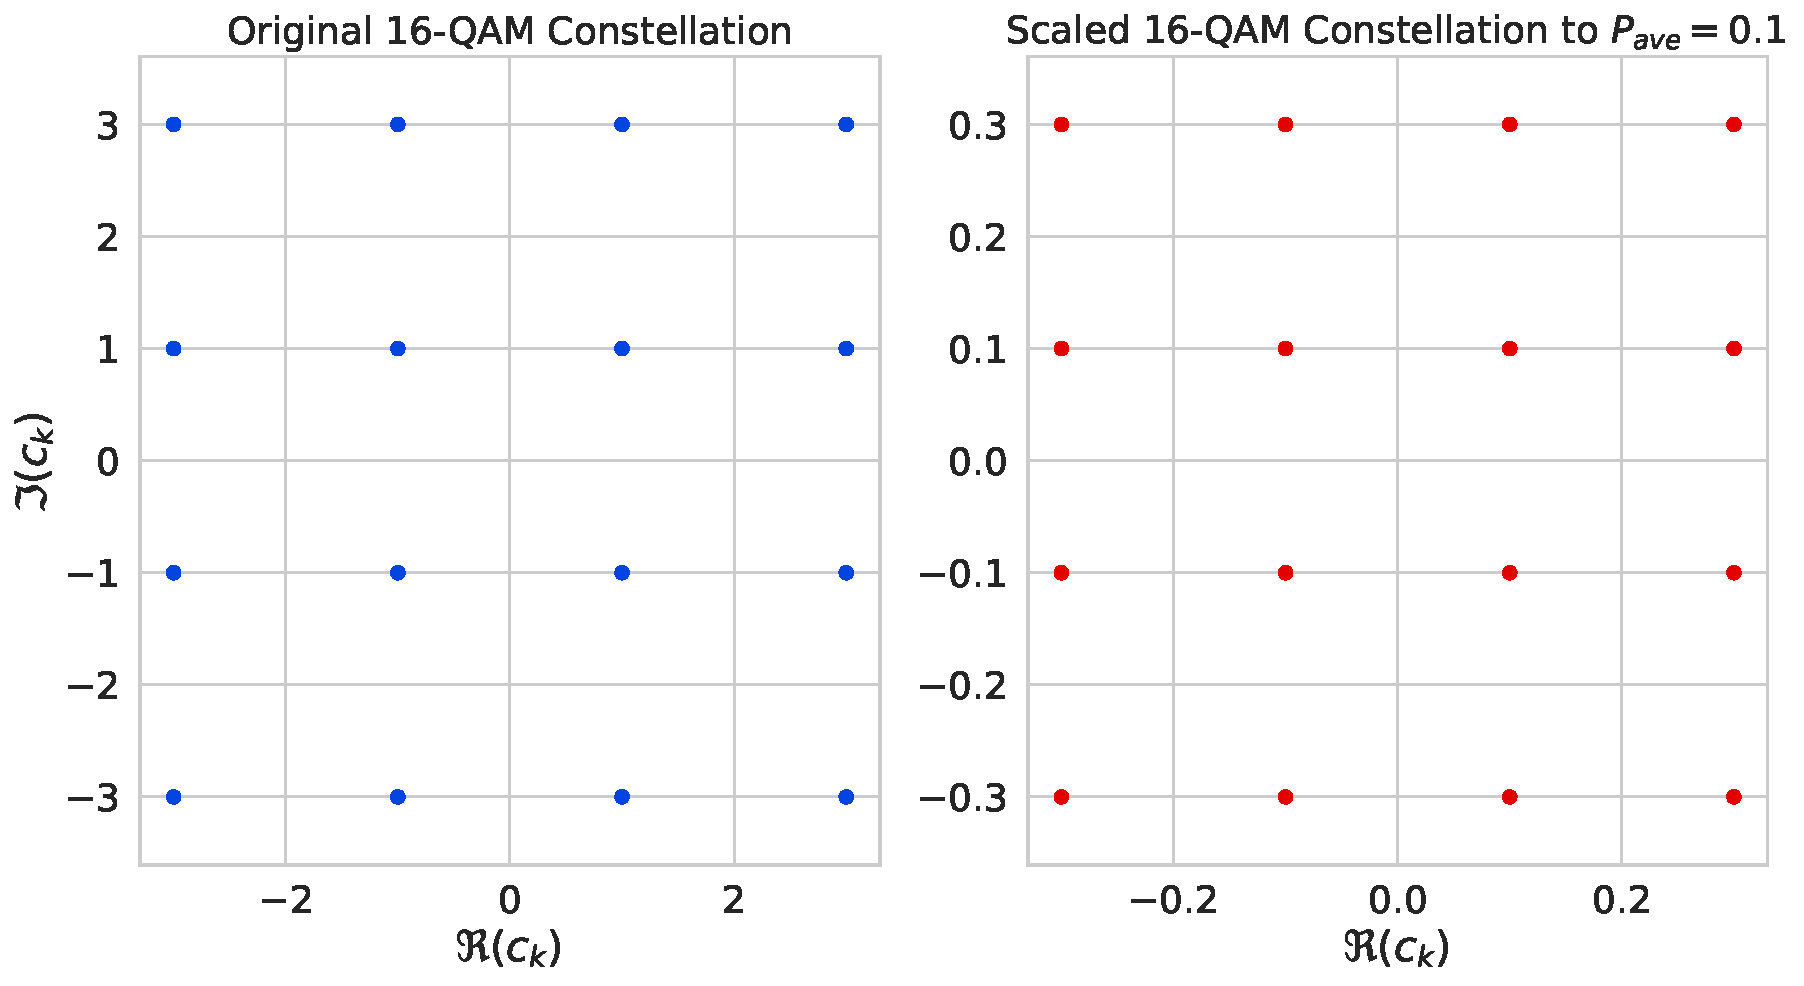
\includegraphics[width=1.0\linewidth]{images/hpcom/constellation_scale.pdf}
    }
    \caption{A visualization displaying two sets of 16-QAM constellations on a complex plane. The left plot shows the original constellation, marked in blue, where each point represents a unique symbol. The right plot illustrates the scaled constellation, colored in red, which has been normalized to achieve a specified average power level of 0.1.}
    \label{fig:constellation_scale}
\end{figure}

Constellation points normalization is a technique used in digital signal processing, specifically in the context of modulation in communications, to ensure that the average power of the constellation points matches a desired level. This process is particularly important in systems like Wavelength Division Multiplexing (WDM), where each signal's power needs to be controlled to avoid interference and optimize the transmission.

The average power of a constellation is computed as the mean of the squared magnitudes of all the constellation points. In the Python code provided, the constellation points are obtained and then scaled to match the desired average power, $P_{ave}$, which is an attribute of the WDM system.

The scaling factor is derived by dividing the square root of $P_{ave}$ by the square root of the actual average power of the unscaled constellation. This ensures that after scaling, the constellation will have the required average power. The functions \texttt{get\_scale\_coef\_constellation} and \texttt{get\_sq\_of\_average\_power} are used to compute the scaling factor based on the modulation type.

Let $c_k$ represent the constellation points for a given modulation scheme, and $P_{\text{ave}}$ denote the desired average power for the Wavelength Division Multiplexing (WDM) system. The scaling process can be expressed as:

\[
c_{k,\text{scaled}} = c_k \cdot \frac{\sqrt{P_{\text{ave}}}}{\sigma_{c}}
\]

where $\sigma_{c}$ is the scaling factor for constellation and defined as:

\[
\sigma_{c} = \sqrt{\frac{1}{N} \sum_{i=1}^{N} |c_i|^2}
\]

Here, $N$ is the number of constellation points, and $|c_i|$ is the magnitude of the $i$-th constellation point. This normalization ensures that the average power of the constellation is equal to $P_{\text{ave}}$.

The value 
\[
\frac{\sqrt{P_{\text{ave}}}}{\sigma_{c}}
\]
is the scaling coefficient that is used to adjust the constellation from a standard scale (as shown in Fig.~\ref{fig:constellation_scale}) to the desired power level.


\section{Simulation Script for Data Mining}
% \begin{lstlisting}[language=Python,caption=Python example,label=lst:example]
% def hello_world():
%     print("Hello, World!")
% \end{lstlisting}

The script~\ref{lst:data_collection} serves as a detailed example of simulating and analyzing optical communication systems. It begins by importing necessary libraries such as TensorFlow for GPU memory management, Pandas for data handling, and HpCom for signal generation and channel modeling. By specifying a directory for data storage and a job name, it ensures organized handling of different simulation batches. The script outlines a variety of system, signal, and channel parameters, setting the stage for a range of simulation scenarios. Through nested loops, it iterates over various configurations of these parameters, each time setting up the signal and channel conditions, running the simulation, and collecting key metrics like bit error rate and Q-factor, along with the transmitted and received points. This data is compiled into a Pandas DataFrame, which is then saved to a Pickle file for each set of channel count and average power values, ensuring organized storage of simulation outcomes. The script also demonstrates efficient management of GPU memory allocation, which is crucial in multi-GPU setups. By conducting multiple runs with identical parameters, it accumulates a significant amount of data, addressing the limitations posed by restricted GPU memory. A 'done' message at the end signifies the successful completion of the script, exemplifying a structured approach to exploring and analyzing various configurations in optical communication systems. This script can serve as a robust framework for those looking to conduct thorough analyses of optical communication systems under varying conditions.

\lstinputlisting[
    language=Python,
    caption=Example of data generation for range of parameters,
    label=lst:data_collection
]{code/data_collection.py}


% \section{Something}

% \lstinputlisting[
%     language=Python,
%     caption=Example,
%     label=lst:example
% ]{code/create_wdm_parameters.py}